\section{Implemented Tool} \label{sec:implemented-tool}
\subsection{Overview}
The system referenced in Section \ref{sec:novel-contributions} and especially in Subsection \ref{subsec:interfacing-user}, is a proof of concept terminal-based software tool that was developed in order to test the hypotheses referenced in the \nameref{sec:introduction-results} to this chapter and laid out in Sections \ref{sec:response} and \ref{sec:methodology-introduction}.
The whole software tool has been made freely available for research purposes\footnote{\url{https://github.com/Tioz90/Bayesian-Networks-Explainability-Tool}}.
The major goal in the creation of such a tool is to have a working software that could be given to a number of clinicians at the ICP (see Subsection \ref{subsec:istituto-cantonale}) in order to carry out the research program defined in Section \ref{sec:response}, which is a response to the gaps identified in Chapter \ref{chap:literature-review}.
This being only a prototype, the implementation was carried out using Python, as this was the language that enabled the best focus on rapid development, due to its familiarity and to its vast array of available libraries.

Despite never having been intended to be production software, particular care was taken in the design of the interfacing methods, as described in Subsection \ref{subsec:interfacing-user}, in line with the spirit of this work that is to study human-machine interaction.

In the following section, the various interaction modes that were developed are presented using screenshots.
The basic methods underlying the software tool have already been discussed at length in Section \ref{sec:novel-contributions} so the current examination will focus on the user interface and how these methods have been incorporated into the system.
Where relevant, the information and descriptions given in Section \ref{sec:novel-contributions} will be integrated.

Figure \ref{fig:sw_0} shows the initial screen presented during use.
The user can input the path to the data set to use or can accept the hardcoded one, which in this case is the one described in Section \ref{sec:data-set}.
Next, the number of entries before and after preprocessing are shown; the data set in question sees its number of valid records go from 3217 to 2873, after the rules summarised in Table \ref{tab:datasetpreprocess} have been applied.
The \enquote{Inspect data set} and \enquote{ML} options are only for testing purposes; the former surfaces a pair of options to visualise the distribution of the data set's variables' values and their normalised entropies, the latter runs a series of tests that will not be discussed.
%the latter runs the machine learning tests that will be discussed in Section \ref{sec:bn-prediction-evaluation}.

The user-oriented section of the software is the one accessed by selecting \enquote{Build Bayesian Network}; this is where all the methods discussed in Chapter \ref{chap:methodology} are to be found and will be the object of the present evaluation.
Selecting this option automatically uses the Pomegranate package to construct a Bayesian network model using the previously selected data set.
The user is then shown the main menu of the application, as can be seen in Figure \ref{fig:sw_1}.

\begin{figure}[htbp]
\centerline{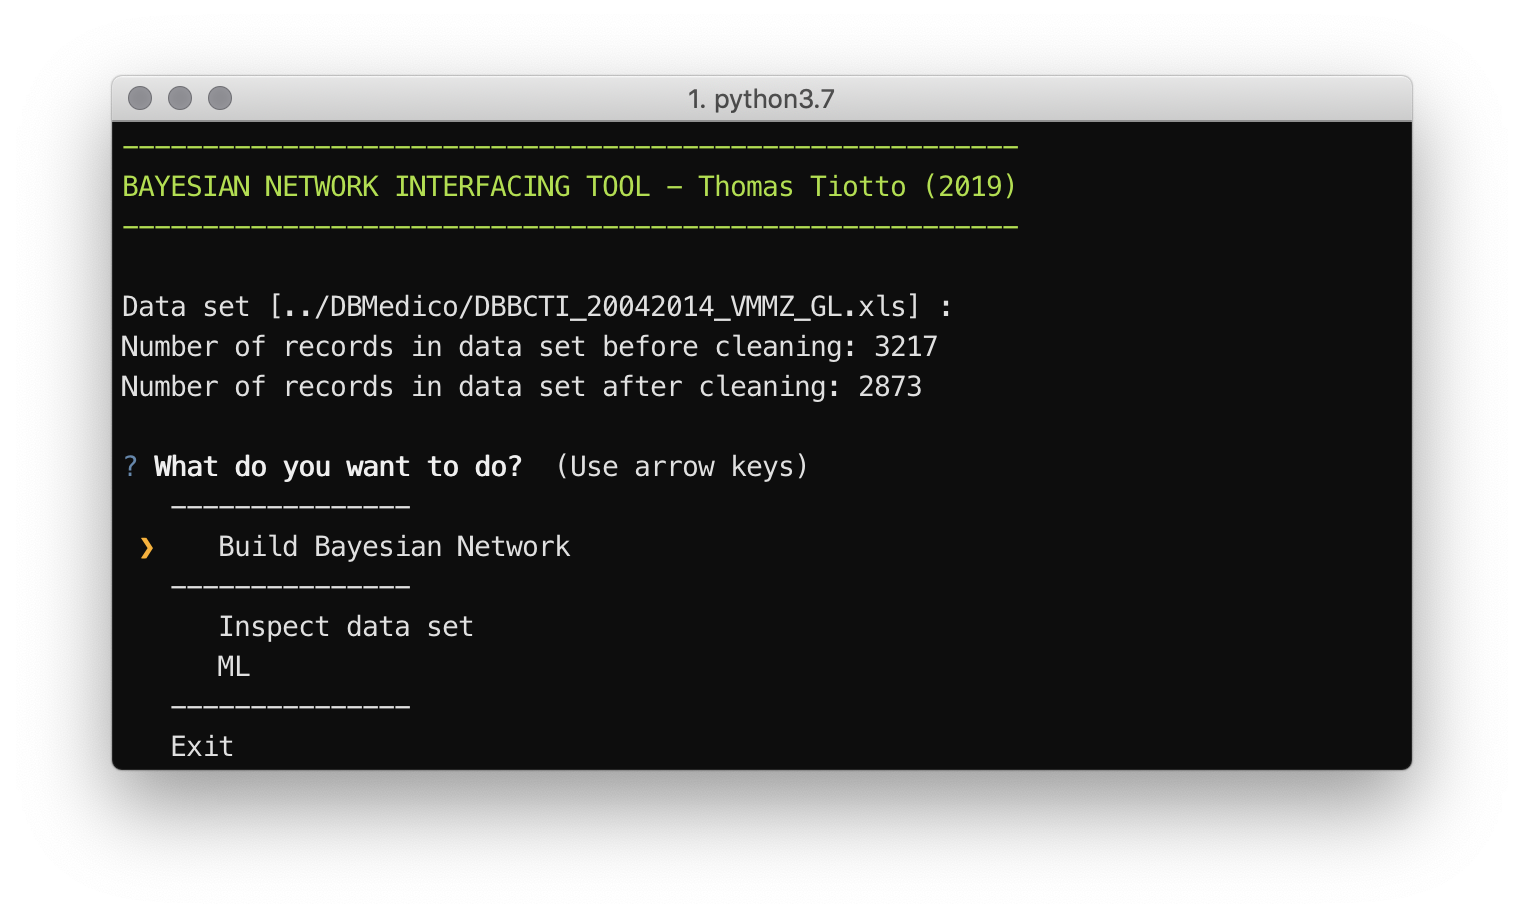
\includegraphics[width=0.7\textwidth]{results/images/sw_0}}
\caption{Initial screen in the developed tool.}
\label{fig:sw_0}
\end{figure}

\begin{figure}[htbp]
\centerline{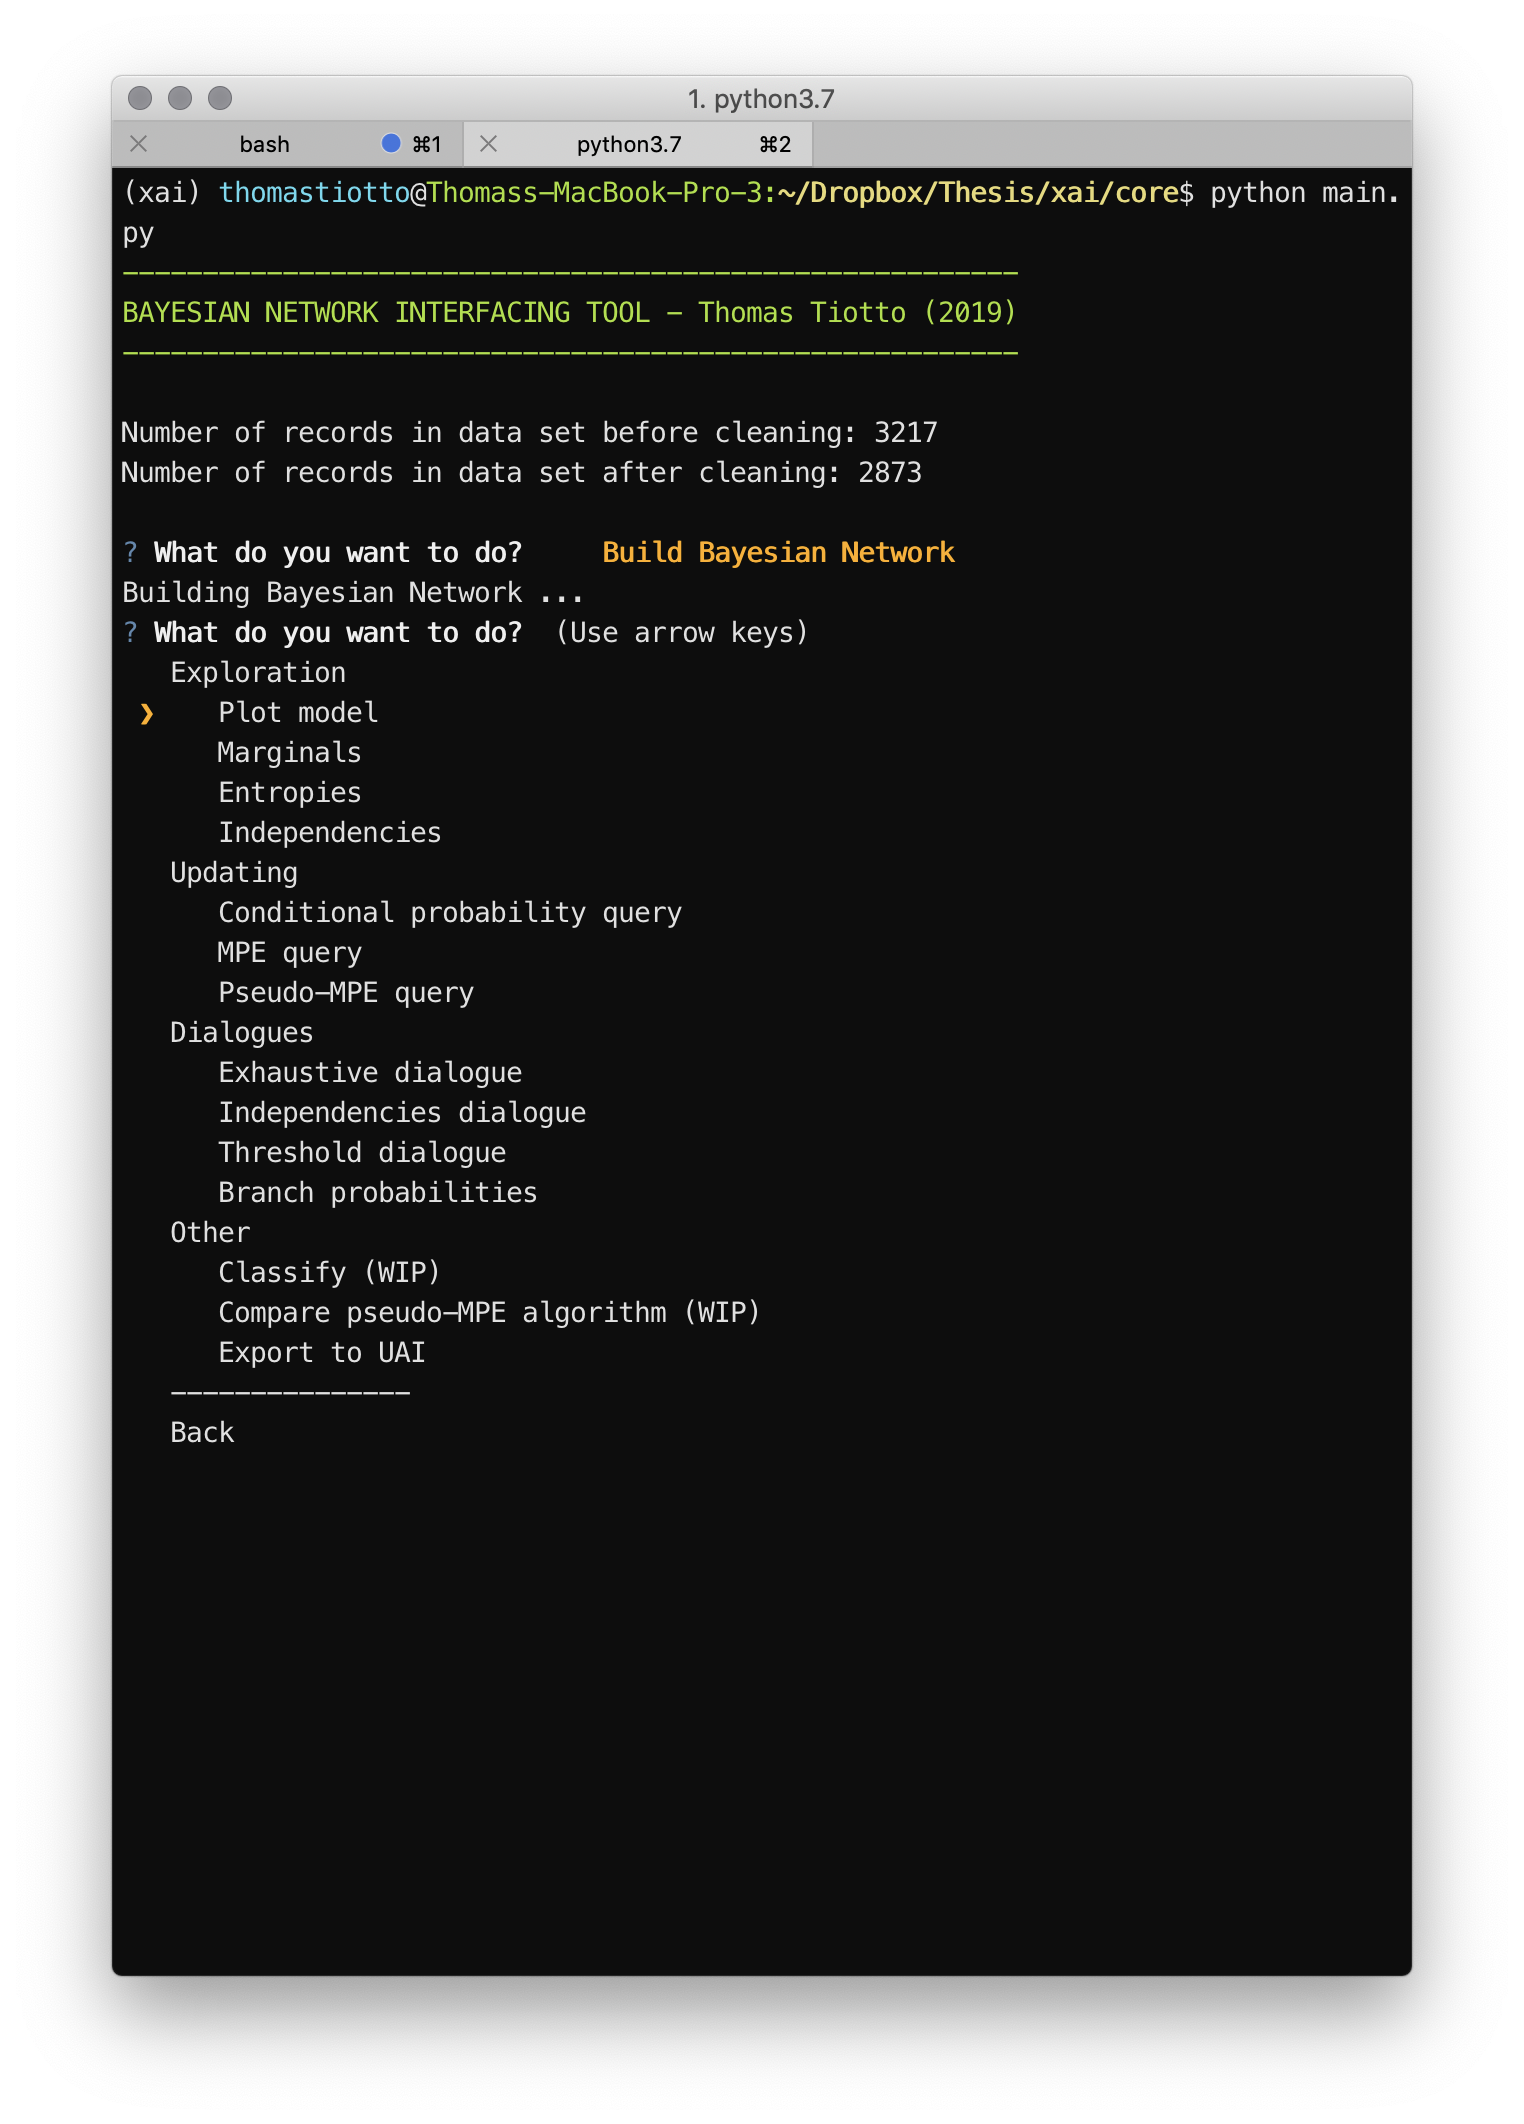
\includegraphics[width=0.7\textwidth]{results/images/sw_1}}
\caption{Main interaction menu.}
\label{fig:sw_1}
\end{figure}

\subsection{Plot Model}
The \enquote{Plot Model} interaction mode would be an example of a \textit{static}, \textit{graphical} explanation in the framework defined by \citet{lacave2002review}, aimed at \textit{explaining the model}.
Compared to the characteristics of an explanation identified by \citet{miller2018explanation}, this might be erroneously regarded as a \textit{causal} explanation. 
Yet, it is important to remember that the directed graphs underlying a Bayesian network are not necessarily describing causal relations, but only probabilistic dependencies.

The \enquote{Plot model} interaction mode gives the expert an overview of the variables present in the system and their relationships by displaying the underlying BN's DAG, with the directionality of edges removed for the reasons explained in \ref{subsec:results-independencies-dialogue}.
Apart from the DAG, mutual information (Definition \ref{def:mutual-information}) between every pair of connected variables is shown on the edges in order to help the expert gauge the strength of the connection.

The users at the ICP considered this interaction modality a good solution to immediately visualise all the features of the data set at a high level together with their relationships; i.e., it gave the user a sense of the \textit{context} of the data set at hand. 
The scaling of the thickness of an edge in a manner proportional to the mutual information of the variables it connects was also considered useful in helping to appreciate the varying strength of the correlations between clinical variables.

The output for the data set presented in Section \ref{sec:data-set} in shown in Figure \ref{fig:sw_plot_result}.

\begin{figure}[htbp]
\centerline{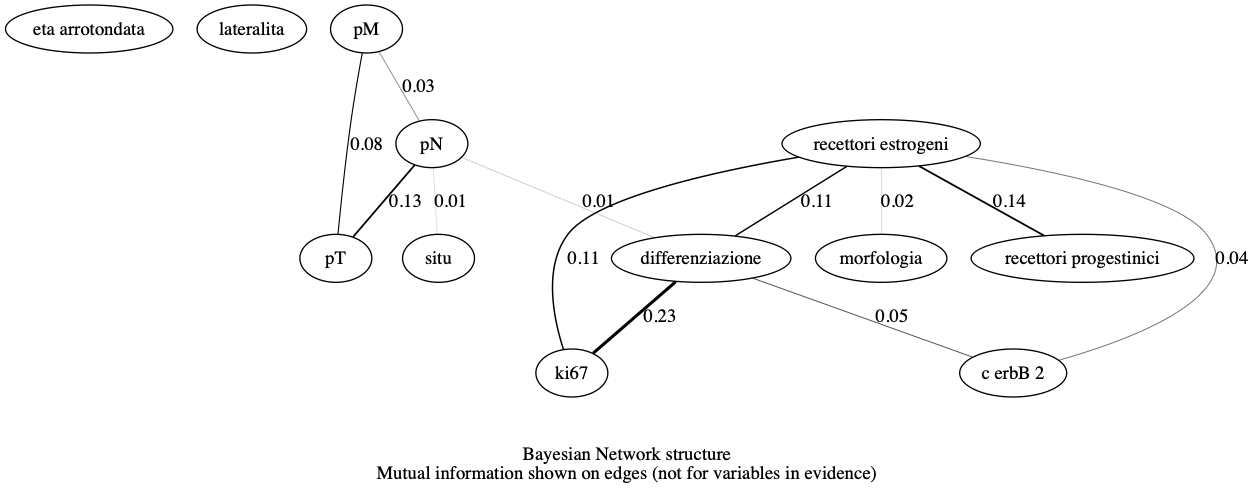
\includegraphics[width=\textwidth]{results/images/plot_result}}
\caption{Plot model output.}
\label{fig:sw_plot_result}
\end{figure}

\subsection{Independencies} \label{subsec:results-independencies-query}
The \enquote{Independencies} interaction mode would be an example of a \textit{static}, \textit{linguistic} and \textit{graphical} explanation in the framework defined by \citet{lacave2002review} aimed at \textit{explaining the model}.
Compared to the characteristics of an explanation identified by \citet{miller2018explanation}, it could be seen as possessing the \textit{selected} and \textit{causal} elements.

The \enquote{Independencies} interaction mode gives the expert the possibility of verifying which d-separations (Definition \ref{def:d-separation}) exist in the constructed Bayesian network's DAG (Definition \ref{def:dag}) .
The concept of d-separation is here reworded into a higher-level notion of \enquote{choosing a source variable and a set of evidence to see which other variables have influence on the source, given the evidence}.
This recasting was deemed necessary because the clinicians at the ICP initially had difficulty in conceptualising at the level of graph theory, probably due to the the misinterpretation of the directionality of the edges in the graphs of a Bayesian network.
Graphs and trees are quite widely-used in clinical practice; however, the presence of an edge is commonly interpreted not as a correlation, but often as an indication of causality. 
Thus, the concept of d-separation could be misinterpreted because of this consolidated viewpoint.
For this same reason, after having chosen first the source variable and then the observed set of evidence variables, the user is presented with an output both in graph (Figure \ref{fig:independencies_output}) and in natural language (Figure \ref{fig:sw_2_independencies}) form.
Having both output modalities present was seen to reduce the confusion that users trained in the medical sciences felt for such an unfamiliar concept.

The new visualisation of d-separation (see Figure \ref{fig:independencies_dialogue_output}), introduced on the basis the the ICP's suggestions, was confirmed by the clinicians to be very intuitive, especially when compared to the initial design (see Figure \ref{fig:independencies_dialogue_output_old}).

\begin{figure}[htbp]
\centerline{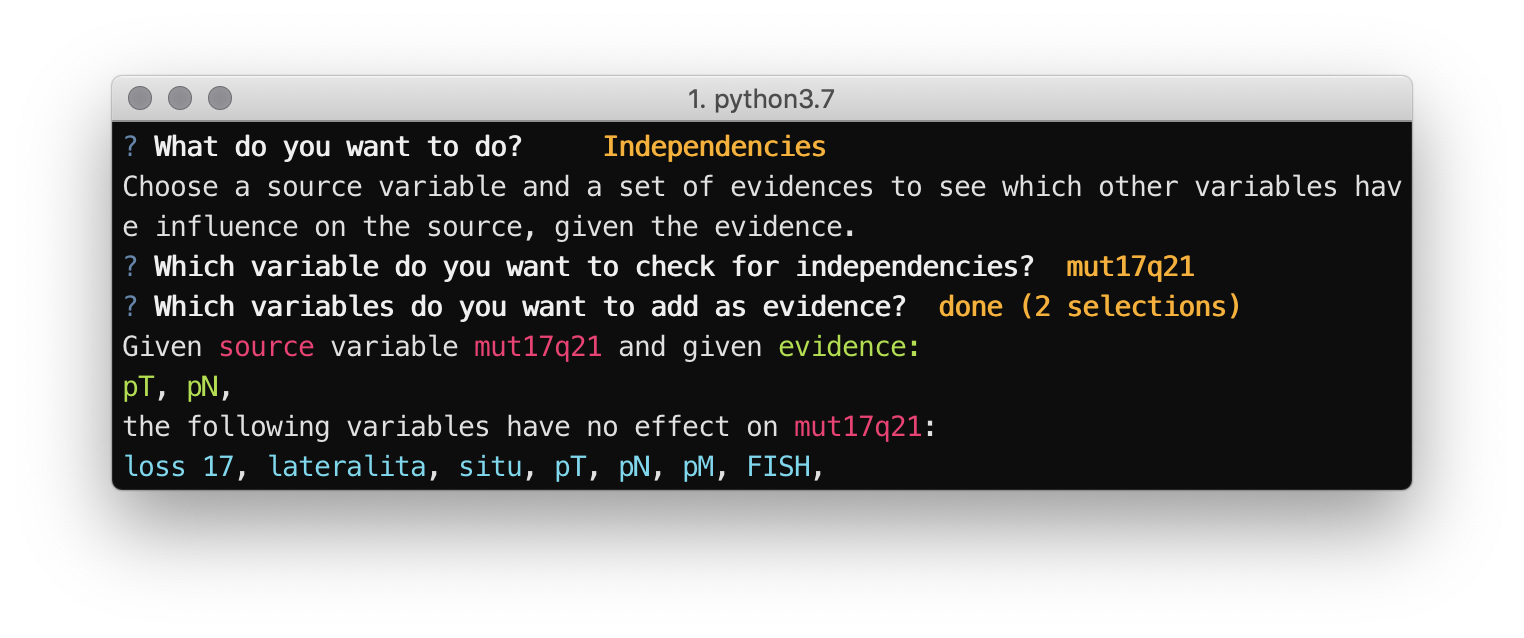
\includegraphics[width=0.7\textwidth]{results/images/sw_2_independencies}}
\caption{Independencies query natural language output.}
\label{fig:sw_2_independencies}
\end{figure}

\begin{figure}[htbp]
\centerline{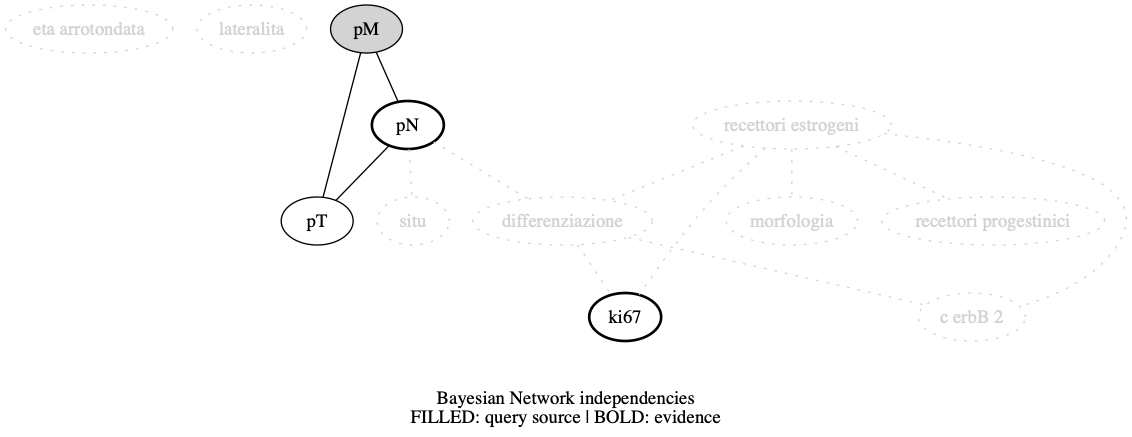
\includegraphics[width=\textwidth]{results/images/independencies_output}}
\caption{Independencies query graph output.}
\label{fig:independencies_output}
\end{figure}

\subsection{Conditional Probability Query} \label{subsec:results-conditional-probability-query}
The \enquote{Conditional Probability Query} would be an example of a \textit{static}, \textit{linguistic} explanation in the framework defined by \citet{lacave2002review} mainly aimed at \textit{explaining the evidence}.
Compared to the characteristics of an explanation identified by \citet{miller2018explanation}, it could be seen as possessing the \textit{selected} element.

Conditional probability queries (Definition \ref{def:conditional-probability}) were seen to be instinctively understood by the clinicians at the ICP.
Indeed, many of the natural language questions that they defined to clinically validate the system (see Subection \ref{subsec:clinical-validation-methodology}) could be framed as and answered by instances of this type of query.

As can be seen in Figure \ref{fig:sw_3_query}, the user is asked for a target variable (in magenta) of which to observe the conditioned values and for a set of variables, together with their observed values (in green).
The output, in natural language, includes all elements of the query together with the colour-coding described in Subsection \ref{subsec:interfacing-user}.
The answer to the question (in cyan), shows the probability of each of the states of the target variable quantified in natural language i.e., as linguistic probabilities, using the coding defined in Table \ref{tab:naturallanguageprobabilities}, and as raw probabilities, shown as percentages.

In addition, the use of colours was appreciated by the users at the ICP because they felt that it helped them to orient themselves among the different elements of the query and also to remember how they had posed it.  

\begin{figure}[htbp]
\centerline{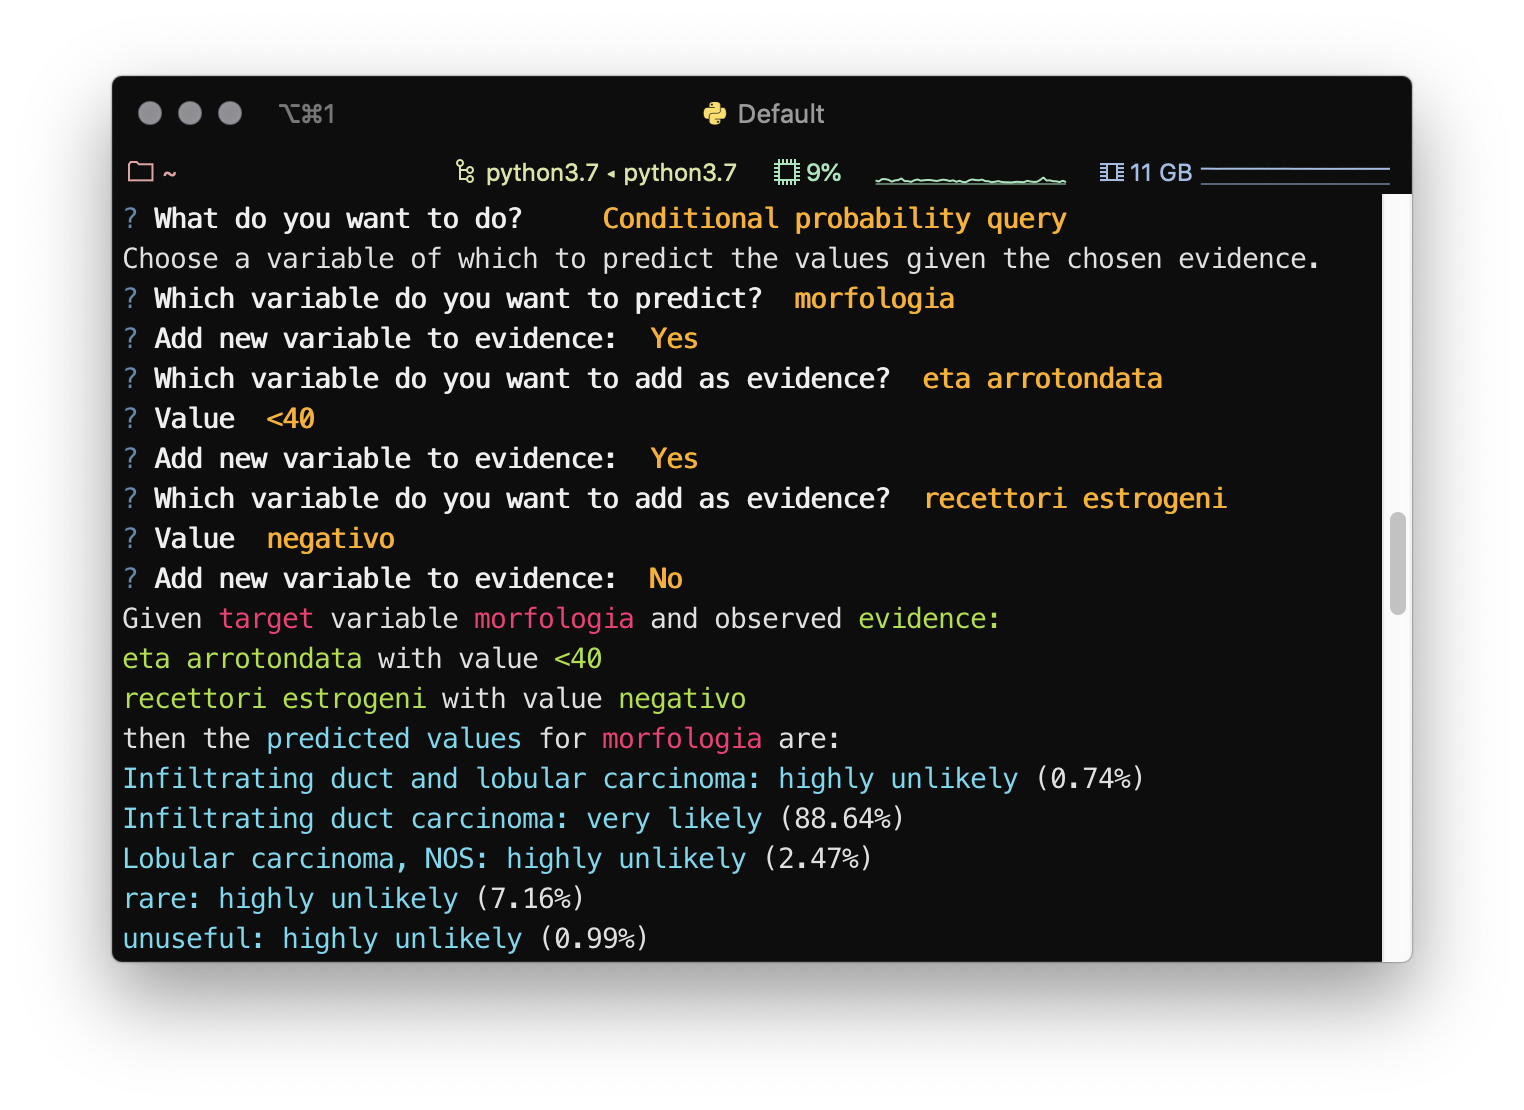
\includegraphics[width=0.7\textwidth]{results/images/sw_3_query}}
\caption{Conditional probability query output.}
\label{fig:sw_3_query}
\end{figure}

\subsection{MPE Query}
The \enquote{MPE Query} would also be an example of a \textit{static}, \textit{linguistic} explanation in the framework defined by \citet{lacave2002review} mainly aimed at \textit{explaining the evidence}.
Compared to the characteristics of an explanation identified by \citet{miller2018explanation}, it could be seen as possessing the \textit{selected} element.

Queries of the MPE type (Definition \ref{def:mpe}) were not initially understood until a bridge to concepts familiar to clinical practitioners had been established.
When presented at an abstract, mathematical level, the experts of the ICP were not sure of the utility of such a query class.
With some work, it was understood that an MPE query could be linked to a concept familiar to any clinician: that of \enquote{a maximally likely patient profile}.
That is, given a set of known parameters it is of interest for the clinician to find which is the most likely assignment to the others.
As each record in the data set represents a patient's clinical profile, this is equivalent to finding the most probable patient given a set of know values.

Another way than an MPE query makes clinical sense, is in the crucial task of predicting missing values for a patient.
This is not an unlikely case, as discussed in Subsection \ref{subsec:motivation}, because there is more than one reason that patients may be missing one or more entries in their clinical profiles.
Executing an MPE query with the known patient's values will yield the most probable assignments to the missing ones and is thus equivalent to a prediction task.
The clinical significance of such an interaction mode can also be inferred from the fact that a number of the natural language questions, that were spontaneously defined to validate the system (see Section \ref{sec:validation}), were seen to map onto instances of this type of query.

At a technical level, the MPE calculation is executed using Pgmpy's \texttt{map\_query} function. 

The output, shown in Figure \ref{fig:sw_4_mpe}, presents, in colour-coded natural language, the input evidence (in green) and most probable assignments to the remaining variables (in cyan).

\begin{figure}[htbp]
\centerline{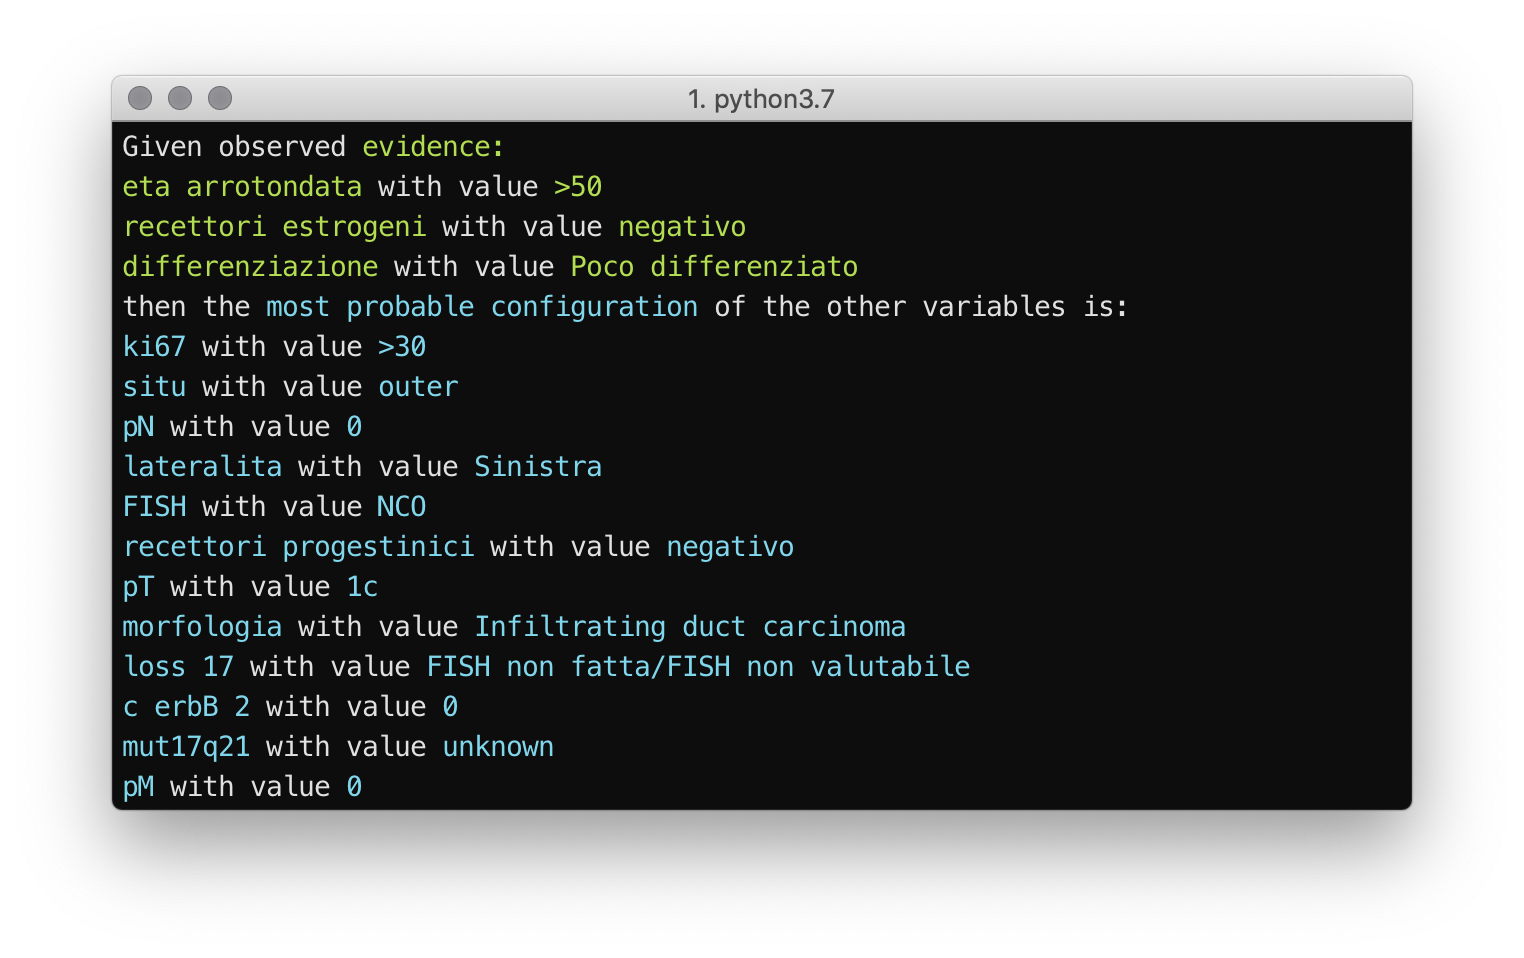
\includegraphics[width=0.7\textwidth]{results/images/sw_4_mpe}}
\caption{MPE query output.}
\label{fig:sw_4_mpe}
\end{figure}

\subsection{Pseudo-MPE Query} \label{subsec:results-pseudo-mpe-query}
The \enquote{Pseudo-MPE Query} would be an example of a \textit{static}, \textit{linguistic} and \textit{graphical} explanation in the framework defined by \citet{lacave2002review} mainly aimed at \textit{explaining the evidence} but also the \textit{reasoning}.
Compared to the characteristics of an explanation identified by \citet{miller2018explanation}, it could be seen as possessing the \textit{selected} and \textit{causal} elements, while remembering that the implications resulting from a BN are not necessarily causal.

The \enquote{pseudo-MPE query} interaction mode is aimed at generating a \enquote{maximally probable} assignment using the methods described in Subsection \ref{subsec:algorithms-novel} under the \enquote{pseudo-MPE from Initial Evidence} header.
The hypothesis is that this should be a valid explainability tool, as it is not only a \textit{linguistic} but also a \textit{graphical} explanation, with the latter element being identified by \citet{lacave2002review} as one of the most effective ways of giving a satisfactory explanation in a BN.\footnote{If the cardinality of the set of variables to explain is one, i.e., $|E| = |V|-1$, with $E$ the evidence set and $V$ the set of variables in the BN, then the \enquote{pseudo-MPE} and true MPE assignments will be identical.}

The user is first asked for the probability threshold under which to discard the \textit{(state,value)} pairs whose probability is deemed too low.
Then, after being asked for the initial observed evidence, the expert is presented with the constructed polytree (Definition \ref{def:polytree}); an output example can be seen in Figure \ref{fig:pseudo_mpe_output}.
This polytree will have the initial evidence, that the expert specified, as roots and a single chain of \textit{(state,value)} pairs, each one quantified with its probability (in natural language) given all of its ancestors.

A doubt, that presented itself quite early during the ICP's evaluation, concerned the quantification of probabilities in the chain.
The pathologists were unsure of why \textit{(state,value)} pairs appeared before others that had been reported as more probable.
For example, in Figure \ref{fig:pseudo_mpe_output}, \textit{(\enquote{morfologia},\enquote{Infiltrating duct carcinoma})} that is considered \textit{likely} appears before \textit{(\enquote{recettori estrogeni},\enquote{fortemente positivo})} which is considered \enquote{very likely}.
The pathologist's intuition brought her to expect this deduction chain to be monotonically decreasing in probability from the initial evidence (that, as such, is certain).

What turned out to be the point of confusion, was that it was unclear that the probability of every node added to the chain depends on all its ancestors.
In the specific example, \textit{(\enquote{recettori estrogeni},\enquote{fortemente positivo})}'s evidence set also contains \textit{(\enquote{morfologia},\enquote{Infiltrating duct carcinoma})}.
There is thus, mathematically, no reason for the chain to be monotonically decreasing in probability because adding new evidence is liable to boost the likeliness of some unobserved variables.
Returning to the example, the marginal probability $\mathbb{P}((\text{\enquote{recettori estrogeni},\enquote{fortemente positivo}}))$ may very well have been less probable than \enquote{very likely}, maybe it was only \enquote{likely} or even \enquote{unlikely}, but this says nothing about the posterior probability $\mathbb{P}((\text{\enquote{recettori estrogeni},\enquote{fortemente positivo}}) \mid (\text{\enquote{morfologia},\enquote{Infiltrating duct carcinoma}}) )$, which is what the polytree displays.

The unclearness of the chain of inferences is certainly not a point to underestimate, as the hope was for the \enquote{pseudo-MPE} output to be able to clarify the underlying reasoning process of the models and thus help in guiding the expert's through process.
If this reasoning process itself were unclear, this could hardly lead to a good explanation; thus an effort will have to be made to explain the underlying assumptions better, while also being mindful when evaluating if this output mode genuinely presents the characteristics of a good explanation.

\begin{figure}[htbp]
\centerline{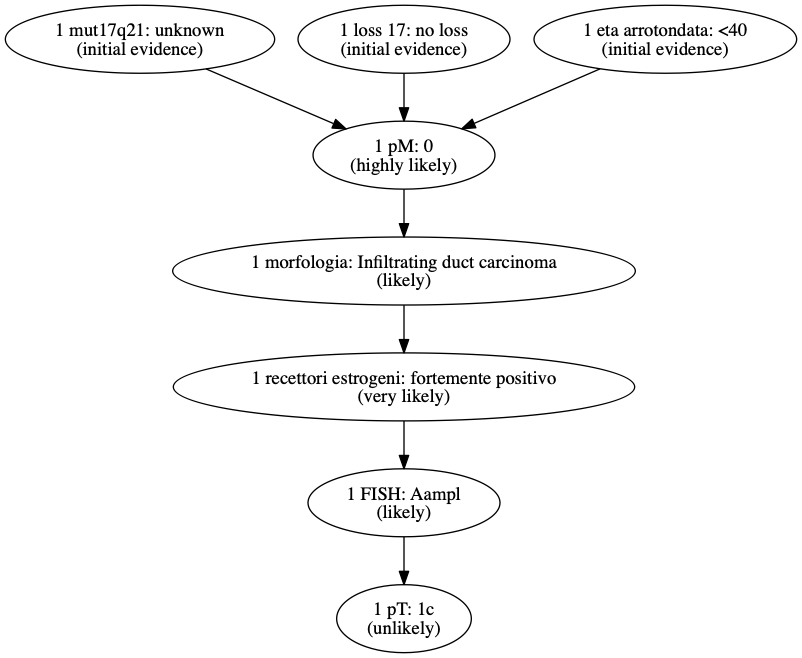
\includegraphics[width=0.7\textwidth]{results/images/pseudo_mpe_output}}
\caption{Pseudo-MPE query output with threshold $0.5$.}
\label{fig:pseudo_mpe_output}
\end{figure}
%
%\subsection{Belief revision}
%\todo[inline]{da lasciare?  da espandere?  da spostare?}
%Philosophically, what is being done during the dialogues is a process of \textit{hard belief revision}.
%This is because the expert's choice is taken by the system as absolute truth and added to the previous evidence set.
%
%The process of \textit{belief revision} is distinct from that of \textit{belief updating} as in the latter previous beliefs are updated to conform to new information received.
%Belief revision on the other hand does not modify previous evidence, as this is simply supposed to be less reliable than the newer one.
%This last setting is the one that happens during the dialogues, because previous \textit{(state,value)} tuples are not modified in their probabilities given the new evidence supplied when the expert accepts a proposal.
%We talk about \textit{hard} belief revision because the new evidence generated by the user is treated as if it were certain - i.e., with probability 1 - and added to the evidence set without creating inconsistencies.
%\todo[inline]{come si potrebbe giustificare?  ha senso tenere il paragrafo?}

\subsection{Exhaustive Dialogue} \label{subsec:dialogue-results}
The three dialogue variants would be examples of \textit{dynamic}, \textit{contrastive}, \textit{linguistic} and \textit{graphical} explanations in the framework defined by \citet{lacave2002review} aimed at \textit{explaining the evidence} but also, and most importantly, to \textit{explaining the reasoning}.
Compared to the characteristics of an explanation identified by \citet{miller2018explanation}, these could be seen as possessing all the necessary elements: \textit{contrastive}, \textit{selected}, \textit{causal} and \textit{social}.

The three \enquote{dialogues} are the most experimental interaction modes and thus also the most alien to a user.
None of the natural language questions defined by the ICP in the form described in Subsection \ref{subsec:clinical-validation-methodology} could be directly mapped onto such a dialogical process.
On the other hand, the dialogue aims to build an \textit{expert-driven MPE approximation} and could thus be regarded as essentially answering the same question as the \enquote{pseudo-MPE} and \enquote{MPE} queries (Subsection \ref{subsec:results-pseudo-mpe-query}).
The research hypothesis is wether this could be a better explainability tool, as it is not only a \textit{linguistic} and \textit{graphical} explanation but also a \textit{dynamic dialogue} that \citet{Hilton1990} and \citet{lacave2002review} identify as a key ingredient in having an effective explanation.
Another important fact is that the dialogues offer a \textit{counterfactual} branch when the expert dissents with the model; \citet{miller2018explanation} singles out being \textit{contrastive} as one of the defining characteristics of an effective explanation, as this feature closely aligns with our expectations of what an explanation should entail.

Because of the novel nature of such a knowledge-extraction process, three different versions were implemented with each one adding a different set of behaviours to the \enquote{exhaustive} version described in this subsection.
This helped in exploring the space of possibilities and aided in understanding which features were preferred by the clinicians of the ICP, both as a means for knowledge-extraction from the data set and from a comprehensibility point of view.
It should here be noted that comprehensibility of the outputs is a \textit{necessary} but \textit{not sufficient condition} to be able to gain knowledge from data.
Both variants to the basic dialogue - the independencies-aware and the thresholded one - aim to prune the space of variables proposed to the user in order to reduce her cognitive load.
This is in keeping with the insight by \citet{miller2018explanation} that explanations are \textit{selected}, meaning that we humans expect that the explaining factors be picked based on some criterion.

The \enquote{exhaustive dialogue}, as described in much more detail in Subsection \ref{subsec:algorithms-novel} under the \enquote{Dialogues} header, is so named because it ends only when the expert user has reviewed all the variables present in the data set.
It starts by asking the clinician for a set of initial evidence and from thereon after iteratively proposes the \textit{(state,value)} pair with the least entropic \textit{state}, based on the accumulated evidence (the rationale behind this is explained in Subsection \ref{subsec:entropy-based-selection}).
An example of such an ongoing interaction is shown in Figure \ref{fig:sw_5_exhaustive_dialogue}.

An issue that was highlighted early on was that the experts had great trouble in building the \textit{knowledge base} from a single evidence; this was the driving motive that pushed the representation of the \enquote{pseudo-MPE} branch beyond a simple \textit{tree} (Definition \ref{def:tree}) - as in \citep{Butz2018} - but towards a \textit{polytree} (Definition \ref{def:polytree}).
This way the expert is able to inject the query with as much domain knowledge as she feels comfortable with.
It was an unrealistic assumption to expect a domain expert to bear the cognitive load of selecting a \textit{single best initial evidence}; this would be a hard task to do in its own right but it is made even more difficult by the fact that the subsequent dialogue \textit{depends} on the initial evidence.
To effectively select one best evidence, the expert should also have been able to \textit{predict} how the dialogue would have evolved from that initial point onwards.
The dialogue is an \textit{exploratory tool} that the user utilises with the objective of extracting knowledge from the data set; expecting the user to already know the outcome of her choices would mean that she already had the domain knowledge necessary to predict the consequences of those same choices; a clear instance of \textit{circular reasoning}.
This was confirmed by the ICP: having multiple initial evidence helped the users because it reduced the number of tuples proposed by the system and therefore the quantity of choices the users were tasked to deal with.

The general feeling being echoed by the users at the ICP was that the dialogue was the hardest interaction mode to understand and to utilise.
The way they used the dialogues was by nearly always replying \enquote{yes} to its proposals, because they were mostly interested in seeing what the machine would propose.
Nonetheless, the users understood the high potential of this method especially when applied with the objective of conducting research, but they reported they would need to \enquote{trust} the interaction mode before feeling comfortable with using it in such a manner.
They felt that probably having more time to experiment with this kind of interaction might improve their confidence felt in using it, that was lower than that perceived for the other interaction methods.

\begin{figure}[htbp]
\centerline{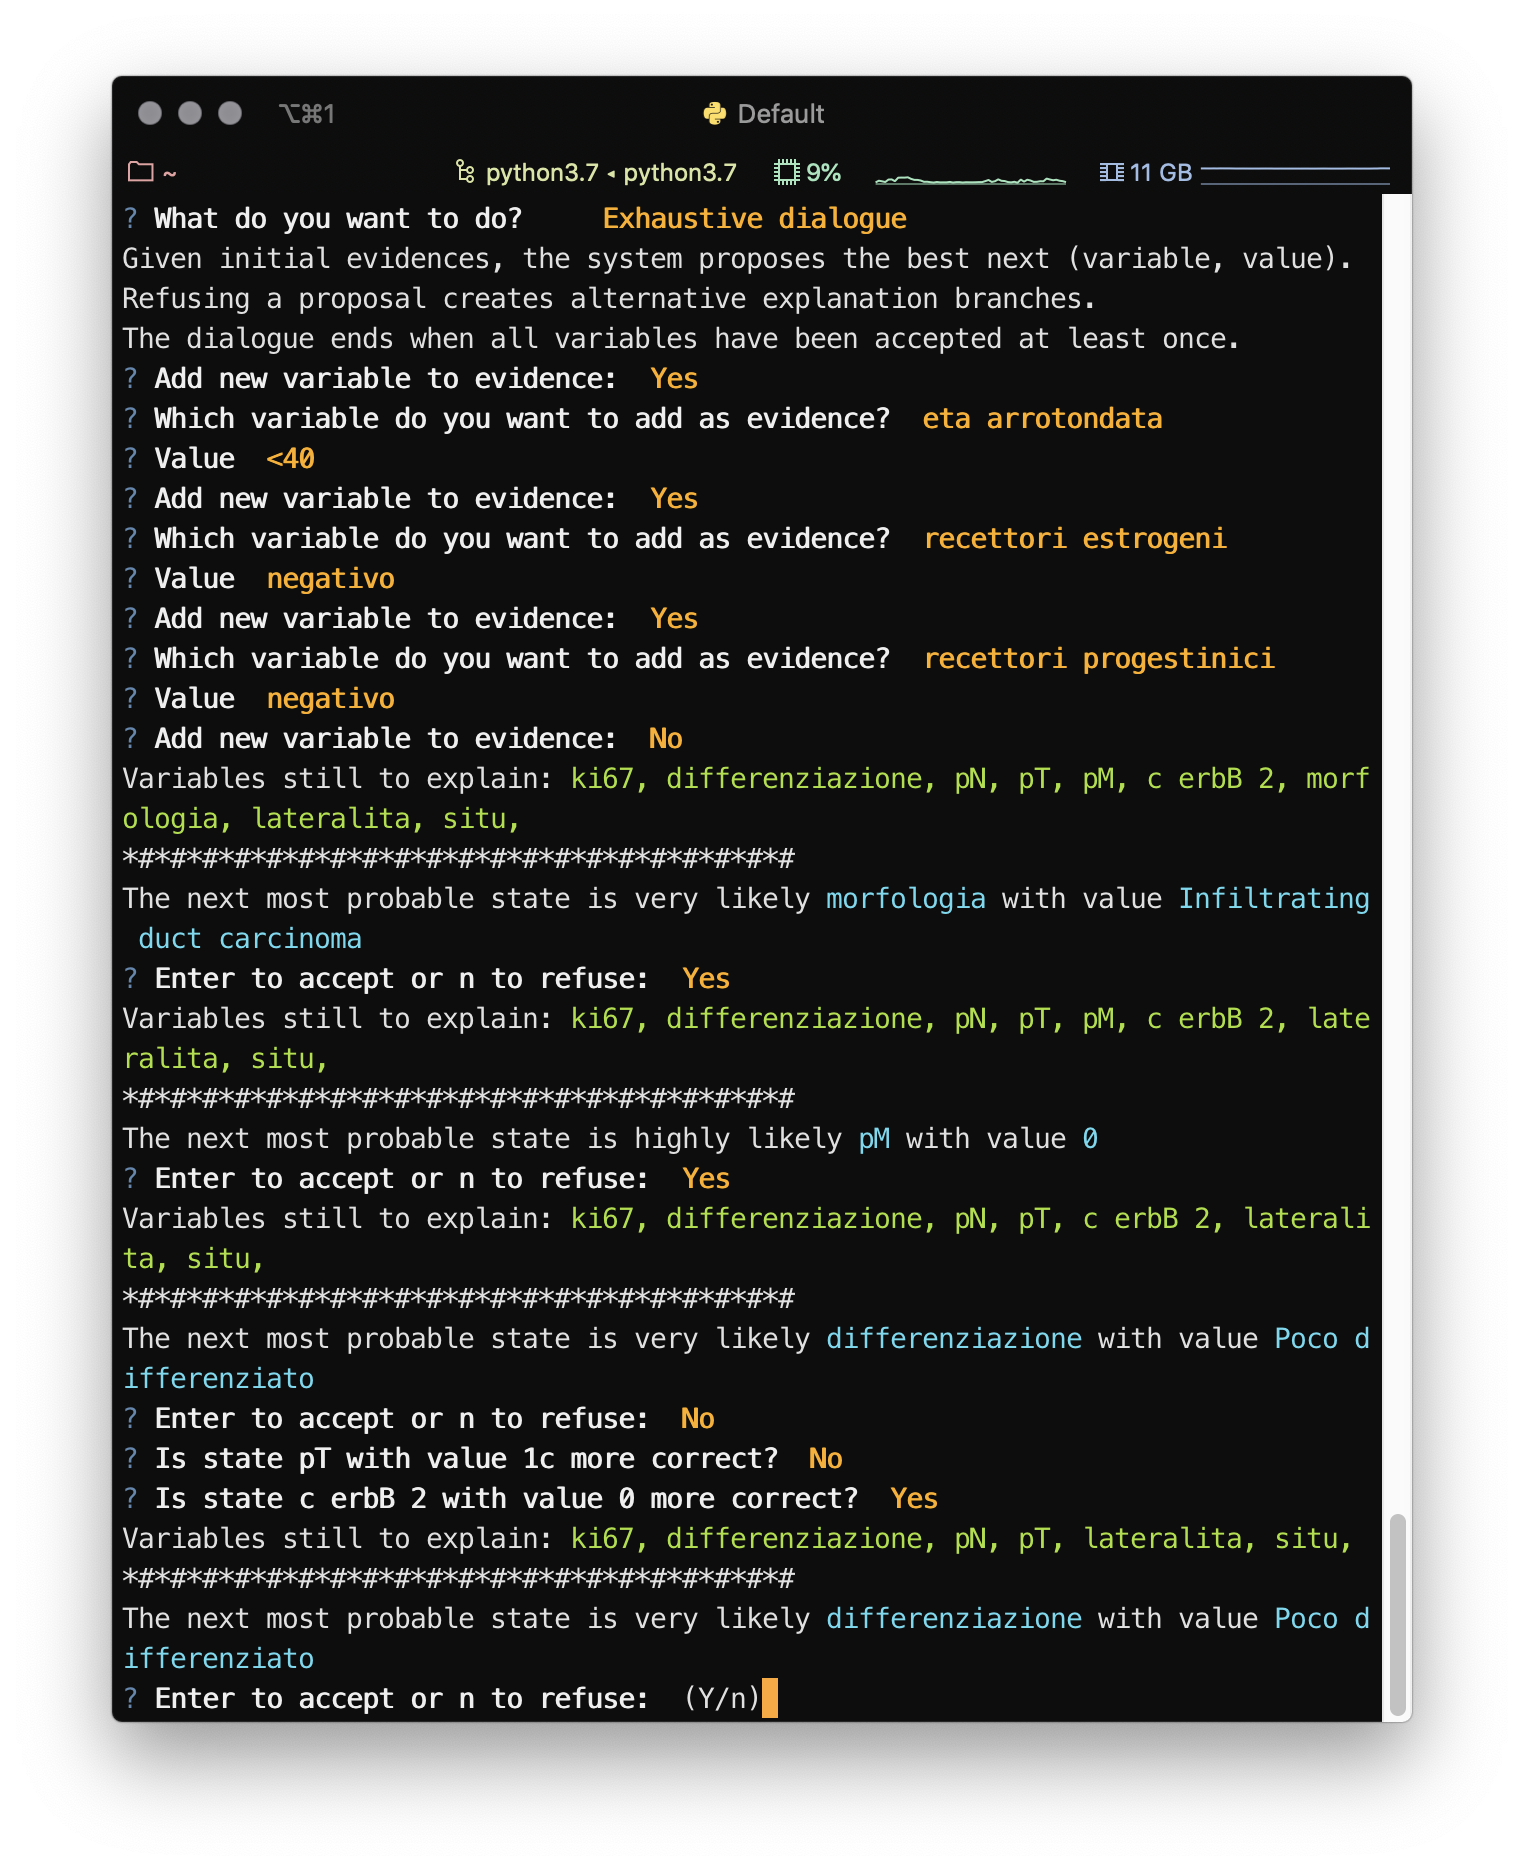
\includegraphics[width=0.7\textwidth]{results/images/sw_5_exhaustive_dialogue}}
\caption{Ongoing Exhaustive Dialogue.}
\label{fig:sw_5_exhaustive_dialogue}
\end{figure}

\subsection{Independencies Dialogue} \label{subsec:results-independencies-dialogue}
The first variant to the \enquote{exhaustive dialogue} takes the approach of excluding variables based on their d-separation properties (Definition \ref{def:d-separation}) in the underlying DAG (Definition \ref{def:dag}).
Thus the cardinality of the set of variables proposed to the user varies in a non-linear way, depending on the topology of the graph and the order of insertions into the evidence set.
In the \enquote{exhaustive dialogue}, presented under the previous header, the relationship between the set of variables still to explain at step $t$, $W_t = V \setminus E_t$, with $V$ all the variables and $E_t$ those already added to evidence, obeys the recurrence relation:
\begin{align}
\begin{split}
		W_0 := V, \\
	E_0 := \emptyset, \\
	|W_{t+1}| = |W_t| - 1, \\
	|E_{t+1}| = |E_t| + 1.
\end{split}
\end{align}
That is, at each step $t$ of the \enquote{exhaustive dialogue}, one variable moves from the set still to explain $W$ to the explained one $E$ i.e., after any iteration step, the number of instantiated variables increases by one unit, while the number of variables to explain also decreases by one.
In the \enquote{independencies dialogue}, this relationship depends on the set of variables $Z$ that are d-separated from those already in $E$.
The relationship between the cardinalities is modelled by an operator $\zeta$ that is unique to the DAG of the BN (or to any \textit{i-equivalent}\footnote{I-equivalence identifies classes of graphs that present the same d-separation properties.} one):
\begin{align}
\begin{split}
	W_0 := V, \\
	E_0 := \emptyset, \\
	|W_{t+1}| = \zeta(|E_t|), \\
	|E_{t+1}| = |E_t| + 1.
\end{split}
\end{align}
As d-separation is not monotonic (adding a variable to $E$ may open new paths and d-connect new variables), the cardinality of the set $W$ may vary, from the point of view of the user, in an unpredictable manner.
To attempt to offset this effect, during the dialogue the user is supported by an updated view of the independencies in the graph (an example during the dialogue is shown in Figure \ref{fig:independencies_dialogue_output}).

Before receiving feedback from the ICP, the visualisation of the independencies was the one shown in Figure \ref{fig:independencies_dialogue_output_old}.
The most striking difference was the use of colour-coding to identify the role and the separation of variables with pink identifying the query variables, blue the evidence, red the separated variables and green the connected ones.
As already noted in Subsection \ref{subsec:results-independencies-query}, the concept of d-separation turned out to be quite unfamiliar to the clinicians of the ICP so the first priority was to represent the concept visually in the clearest way possible.
This was achieved, and confirmed in its efficacy by the pathologists, by fading the separated variables and marking those in evidence in bold, as can be seen in Figure \ref{fig:independencies_dialogue_output}.
The fading of separated variables was felt to successfully reinforce the concept of these not influencing the remaining ones and its directness was especially appreciated.

The use of directed arcs to represent the DAG raised another critical issue that hadn't been foreseen.
In the visual representation of a Bayesian network, an arc between two variables represents a correlation between their values while the direction identifies the \textit{parent} and the \textit{child} in the relationship; for example the graphical representation $X \rightarrow Y$ means that $X$ is the parent of $Y$.
This is a defining characteristic of such a model, because the fundamental idea of a BN is to factorise the joint distribution such that each variable's values depend only on that of its parents; the concept of conditional probability table is explained in Section \ref{sec:bayesiannetworks} and some more examples can be seen in Subsection \ref{subsec:algorithms} under the \enquote{MPE} header.
Nonetheless, the pathologists explained that the DAG representing a BN is very similar to diagrams used during clinical research, with the crucial difference that in those a directed arrow represents \textit{causation} and not \textit{correlation}.
In these diagrams a correlative relationship would have usually been represented by an undirected edge.
For this reason the DAG representation of the BN was \textit{disoriented} in all visualisations.
The ICP confirmed that this new formulation was more closely aligned with the intuition that could be expected by a clinician.

The third element of difference, is the addition of the mutual information coefficient (Definition \ref{def:mutual-information}) on the arcs connecting each couple of variables; the coefficient also scales the width of its associated edge, giving further visual feedback to the user.
This functionality was a direct request from the ICP's representatives since after inspecting the initial DAG visualisation they felt the need for a feature that would increase their understanding of the relationships between the variables.
D-separation is binary while mutual information can give the practitioner a much wider (theoretically infinite) range of information.
For example looking at Figure \ref{fig:independencies_dialogue_output} it is quite easy to see that, while \enquote{morfologia} and \enquote{recettori estrogeni} are d-connected, the amount to which they influence each other's values is small compared to other connected variables.
Some arcs are missing the mutual information coefficient because one of the two variables is in the evidence set, e.g., those belonging to \enquote{recettori estrogeni}.

\begin{figure}[htbp]
\centerline{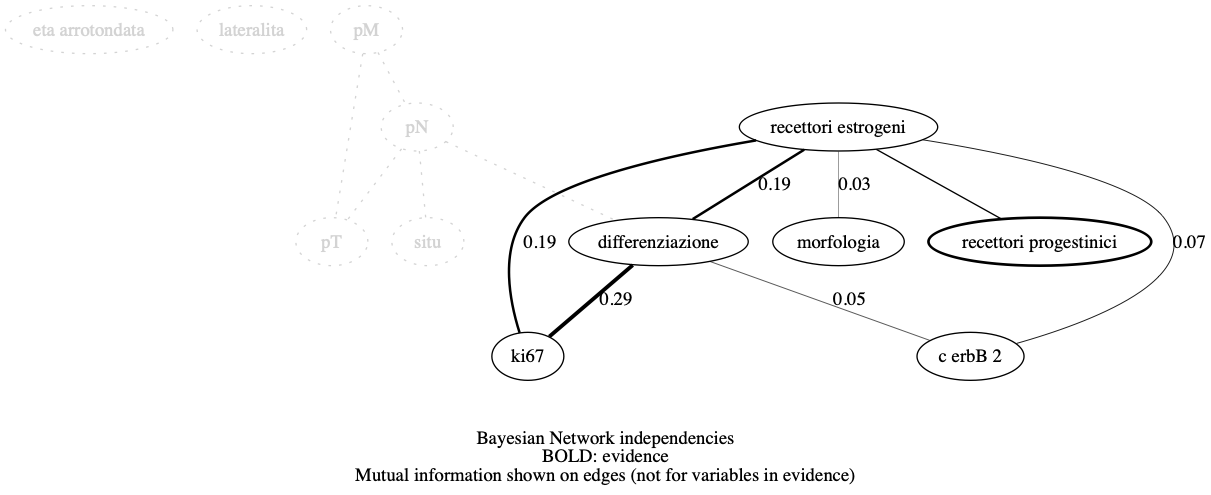
\includegraphics[width=\textwidth]{results/images/independencies_dialogue_output}}
\caption{Ongoing Independencies Dialogue.}
\label{fig:independencies_dialogue_output}
\end{figure}

\begin{figure}[htbp]
\centerline{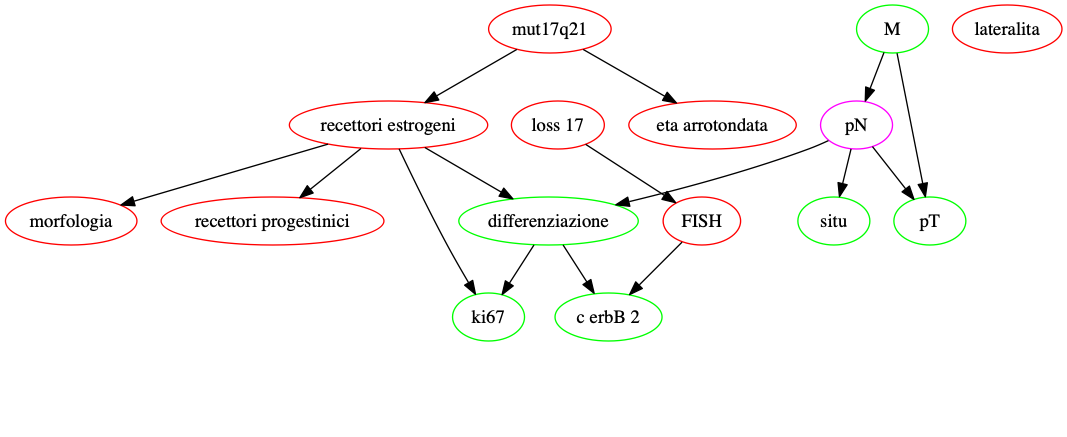
\includegraphics[width=\textwidth]{results/images/independencies_dialogue_output_old}}
\caption{Previous visualisation during Independencies Dialogue.}
\label{fig:independencies_dialogue_output_old}
\end{figure}

\subsection{Thresholded Dialogue}
The final \enquote{dialogue} variant adopts a different strategy for pruning; namely one based on the probability of the proposed tuples and on the number of times they have been refused by the expert.
This implements a suggestion found in \citet{lacave2002review} that explanations should be graded on the user and not on a \textit{fixed user model}; one of the ways this has been addressed in literature is by the introduction of thresholds to filter unwanted information.

The cardinality of the set $W$ of states to explain decreases linearly, similarly to the \enquote{exhaustive dialogue}, but potentially with a slope coefficient $\alpha \leq -1$, as many states may be infra-threshold i.e., too improbable to be considered.
Unlike the independencies dialogue, the cardinality of $W$ cannot increase:
\begin{align}
\begin{split}
	W_0 := V, \\
	E_0 := \emptyset, \\
	|W_{t+1}| = \alpha |W_t|, \\
	|E_{t+1}| = |E_t| + 1.
\end{split}
\end{align}
The default values for the threshold and the maximum number of times a \textit{(state, value)} tuple could be proposed were decided together with the ICP and set to:
\begin{itemize}
  \item \textit{threshold}: 0.4, a \textit{(state, value)} tuple is ignored if the probability of \textit{value} is less that 0.4;
  \item \textit{refusal limit}: 2, a \textit{(state, value)} is ignored if it has already been refused twice.
\end{itemize}